% We switch to portrait mode. This works as advertised.
\documentclass[a0,portrait]{a0poster}
% You might find the 'draft' option to a0 poster useful if you have
% lots of graphics, because they can take some time to process and
% display. (\documentclass[a0,draft]{a0poster})

%\usepackage[utf8]{inputenc}

% Switch off page numbers on a poster, obviously, and section numbers too.
\pagestyle{empty}
\setcounter{secnumdepth}{0}

%fonts
\usepackage[T1]{fontenc}
\usepackage{fontspec}
%\usepackage[oldstylenums, largesmallcaps]{kpfonts}
%\setmainfont[Numbers=OldStyle]{Tex Gyre Pagella}
\setmainfont{Tex Gyre Pagella}
\setsansfont[BoldFont=Lovelo-LineBold]{Lovelo-LineBold}
%\renewcommand*\sfdefault{ugq}

\usepackage{hyperref}
\hypersetup{%
	pdftitle={Wrinkling and nested buckling in a confined protein gel},%the title
	pdfauthor={Mathieu Leocmach},%your name
}

%proper math and math symbols
%\usepackage{amsmath}
\usepackage{amssymb}

\usepackage{siunitx}

\usepackage{multirow}

% Allow the usage of graphics (.jpg, .png, etc.) in the document
\usepackage{graphicx}
\usepackage{tikz}
\usetikzlibrary{arrows,shapes,backgrounds, positioning, intersections, decorations.markings, decorations.shapes, mindmap, shapes.geometric, matrix, patterns}

\usepackage{pgfplots}
%\usepgfplotslibrary{units}
\usepgfplotslibrary{groupplots}
\pgfplotsset{every axis/.append style={xlabel near ticks,ylabel near ticks,mark size={0.2em}}}
\pgfplotsset{every axis plot post/.append style={very thick}}

\usepgfplotslibrary{external}
%\tikzexternalize
%\tikzsetexternalprefix{fig_Rome/}
\tikzset{external/system call={lualatex \tikzexternalcheckshellescape -halt-on-error -interaction=batchmode -jobname "\image" "\texsource"}}

\usepackage{ragged2e}
\RaggedRight

\definecolor{Main}{rgb}{1, 0.57, 0}
\definecolor{Accent1}{rgb}{1,0.28,0}
\definecolor{Accent2}{rgb}{1,0.74,0}

% see documentation for a0poster class for the size options here
\let\Textsize\normalsize
\def\Norulehead#1{\noindent\hbox to \hsize{\hfil\LARGE\textcolor{Main}{\textsf{#1}}}\bigskip}
\def\Head#1{\Norulehead{\dotfill #1}}
\def\LHead#1{\noindent{\LARGE #1}\smallskip}
\def\Subhead#1{\noindent{\large\color{Accent1}\textsc{#1}}}
\def\Title#1{\noindent{\VeryHuge\color{Accent2}\raggedright\textsf{#1}}}

% The textpos package is necessary to position textblocks at arbitary 
% places on the page.
\usepackage[absolute,overlay,showboxes
]{textpos}
% Set up the grid
%
% Note that [40mm,40mm] is the margin round the edge of the page --
% it is _not_ the grid size. That is always defined as 
% PAGE_WIDTH/HGRID and PAGE_HEIGHT/VGRID. In this case we use
% 15 x 25. This gives us a wide central column for text (7 grid
% spacings) and two narrow columns (3 each) at each side for 
% pictures, separated by 1 grid spacing.
%
% Note however that texblocks can be positioned fractionally as well,
% so really any convenient grid size can be used.
%
\TPGrid[40mm,40mm]{15}{25}  % 3 - 1 - 7 - 1 - 3 Columns

% Mess with these as you like
\parindent=0pt
%\parindent=1cm
\parskip=0.5\baselineskip

\usepackage{paralist}

%bibliography
\usepackage{natbib}
\usepackage{bibentry}
\def\newblock{\hskip .11em plus .33em minus .07em}



\newlength{\mylength}

%\includeonly{}

\begin{document}
%\tikzset{every mark/.append style={scale=0.8}}
%\pgfplotsset{every axis/.append style={small}}

\bibliographystyle{notitle}
%\nobibliography{sift}

% Understanding textblocks is the key to being able to do a poster in
% LaTeX. In
%
%    \begin{textblock}{wid}(x,y)
%    ...
%    \end{textblock}
%
% the first argument gives the block width in units of the grid
% cells specified above in \TPGrid; the second gives the (x,y)
% position on the grid, with the y axis pointing down.

% You will have to do a lot of previewing to get everything in the 
% right place.

% This gives good title positioning for a portrait poster.
% Watch out for hyphenation in titles - LaTeX will do it
% but it looks awful.
\begin{textblock}{15}(0,0)
\centering
\Title{
Wrinkling of a confined porous layer
}

\smallskip
\LHead{Mathieu Leocmach, Mathieu Nespoulous, Thomas Gibaud, Sébastien Manneville
}\hfill\texttt{\color{Accent1}mathieu.leocmach@ens-lyon.fr}\\

\LHead{\textsc{Laboratoire de Physique, Ecole Normale Supérieure de Lyon}\hfill\raisebox{-1.5\baselineskip}{
	
\includegraphics[height=2\baselineskip,clip=true, trim=6mm 14mm 6mm 0]{NEW-Logo-ERC-OUTLINE}\quad
	
\includegraphics[height=2\baselineskip]{logo_ums_grand}\quad
	
\includegraphics[height=2\baselineskip]{CNRSfilaire-Q}\quad
	
\includegraphics[height=2\baselineskip]{logo_ens-lyon}
}}

\end{textblock}

\begin{textblock}{3}(0,2.5)
	\Head{Acid-induced gels}
	
	Milk protein solution (4\%w sodium caseinate) acidified by the slow hydrolysis of glucono-$\delta$-lactone (4\%w \textsc{gdl})
	
	\begin{tikzpicture}
	\begin{groupplot}[%
		group style={
			group name=g, group size=1 by 2,
			xticklabels at=edge bottom,
			vertical sep=0,
			},
		xmin=0,xmax=8,
		scale only axis,
		width=\textwidth-4em,
		height=0.3\textwidth,
		extra tick style={grid=major},%
		ylabel absolute, every axis y label/.append style={anchor=base, yshift=1.25em}
		]
	\nextgroupplot[
		ymin=0, ymax=7, ylabel={\textcolor{Accent1}{pH}},
		extra y ticks={4.6}, extra y tick labels={},%
		]
	\addplot+[no marks,Accent1] table[x expr={\thisrowno{0}/3600.+0.05}]{Y189_28800s.pH};
	\node[base left=0] at (axis cs:8,4.6) {isoelectric};

	\nextgroupplot[
		xlabel={time (h)},
		ymin=0, ylabel=\textcolor{Accent2}{$G^\prime$ (\si{\pascal})}
		]
	\addplot+[no marks,Accent2] table[x expr={\thisrowno{0}/3600.+0.05}]{Y235_28800s.prise};
	\end{groupplot}
	\end{tikzpicture}
	
For confocal microscopy we label 10\% of the casein.
\end{textblock}

\begin{textblock}{7}(4,2.5)
	\Head{Sealed cell, spontaneous pattern}
	
	%\Subhead{Side view}\\
	\tikzsetnextfilename{cell_brushes}
	\tikzset{external/force remake}
	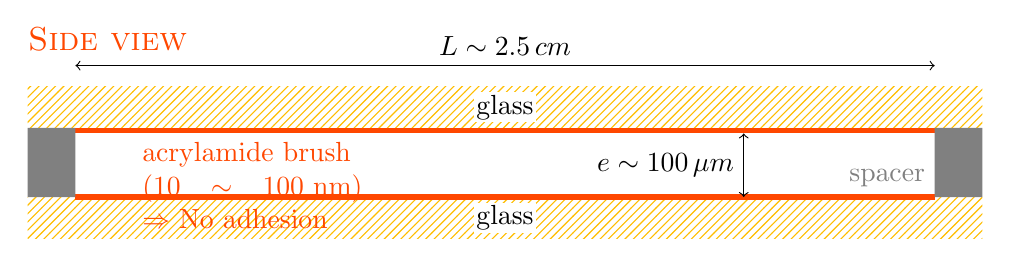
\begin{tikzpicture}
		\fill[pattern=north east lines,pattern color=Accent2] (0,0) rectangle (\textwidth,1.5em) node[midway,fill=white,inner sep=1pt] {glass};
		\fill[pattern=north east lines,pattern color=Accent2] (0,-2.5em) rectangle (\textwidth,-4em) node[midway,fill=white,inner sep=1pt] {glass};
		\draw[line width=2pt,Accent1] (0.05\textwidth,-2.5em) -- (0.95\textwidth,-2.5em) (0.05\textwidth,-1pt) -- (0.95\textwidth,-1pt) node[below,pos=0.30, text width=0.4\textwidth] {acrylamide brush ($10\sim 100$ nm)\linebreak $\Rightarrow$ No adhesion};
		\fill[gray] (0,0) rectangle (0.05\textwidth,-2.5em) (\textwidth,0) rectangle (0.95\textwidth,-2.5em) node[pos=1, above left] {spacer};
		\draw[<->] (0.75\textwidth,-2pt) -- (0.75\textwidth,-2.5em) node[midway,left] {$e\sim 100\,\mu m$};
		\draw[<->] (0.05\textwidth,2.25em) -- (0.95\textwidth,2.25em) node[midway,above] (L){$L\sim 2.5\,cm$};
		\node[anchor=north west, inner sep=0] at ($(L.north) - (0.5\textwidth,0)$) {\Subhead{Side view}};
	\end{tikzpicture}
	
	\Subhead{Top view}\\
	\begin{tikzpicture}[inner sep=0, very thick]
	\setlength{\mylength}{\columnwidth}
	\node[anchor=north west] (a) {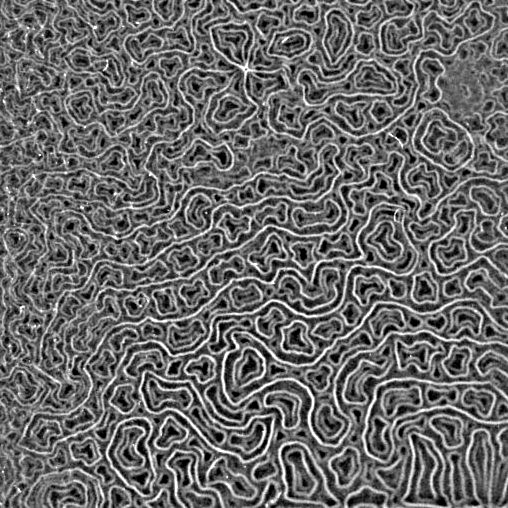
\includegraphics[width=0.28\mylength]{cas3p2_fluo0p8_GDL4_50um_coating_2_zoom2_crop}};
		\node[anchor=north] at (0.44\mylength,0) (b) {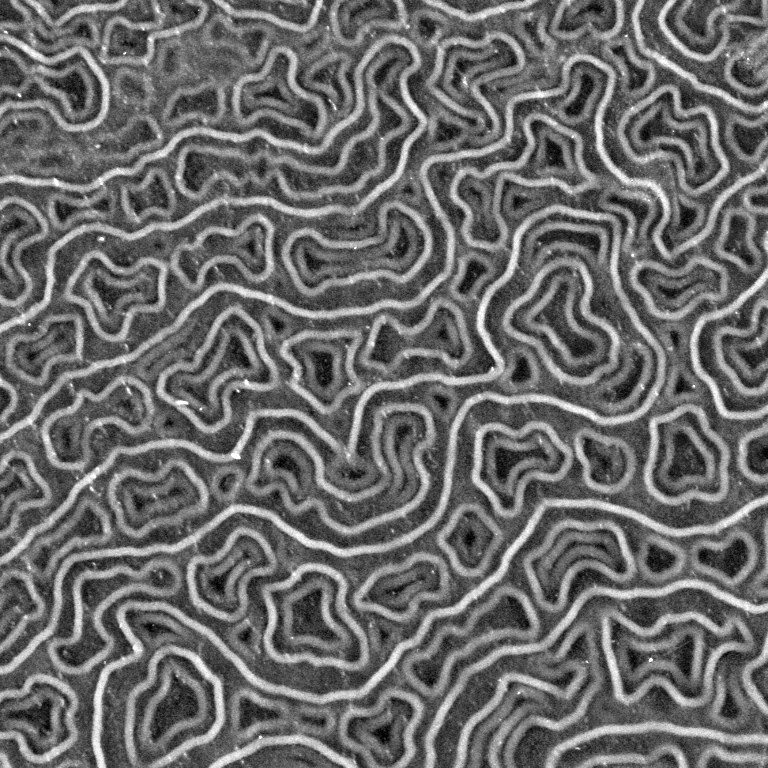
\includegraphics[width=0.28\mylength]{cas3p2_fluo0p8_GDL4_50um_coating_2_zoom6_crop}};
		\node[anchor=north east] at (\mylength,0) (c) {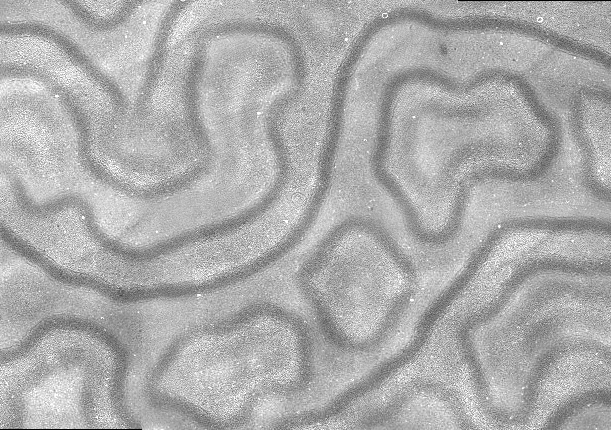
\includegraphics[width=0.4\mylength]{cas3p2_fluo0p8_GDL4_50um_coating_2_transmission}};
		%zooms
		\node[minimum width = 0.137\mylength, minimum height=0.137\mylength, anchor=north west, draw=Accent2] at ($(a.north west) +(0.111\mylength,-0.072\mylength)$) (bz){};
		\draw[Accent2] (bz.north east) -- (b.north west) (bz.south east) -- (b.south west);
		\node[minimum width = 0.128\mylength, minimum height=0.081\mylength, anchor=north west, draw=Main] at ($(b.north west) +(0.097\mylength,-0.143\mylength)$) (cz){};
		\draw[Main] (cz.north east) -- (c.north west) (cz.south east) -- (c.south west);
		\node[minimum width = 0.156\mylength, minimum height=0.156\mylength, anchor=north west, draw=Accent1] at ($(c.north west) + (0.125\mylength,0)$) (dz) {};
		%scale bars
		\draw[ultra thick] (a.south east) ++(0,-0.25em) -- ++(-0.178\mylength,0) node[pos=0.5, below=0.25em, font=\small] (M) {\SI{1}{\centi\metre}};
		\draw[ultra thick] (b.south east) ++(0,-0.25em) -- ++(-0.176\mylength,0) node[pos=0.5, below=0.25em, font=\small] {\SI{5}{\milli\metre}};
		\draw[ultra thick] (c.south east) ++(0,-0.25em) -- ++(-0.132\mylength,0) node[pos=0.5, below=0.25em, font=\small] {\SI{1}{\milli\metre}};
		
		%final volumic view
		%\node[anchor=north east] at (\columnwidth,0) (c) {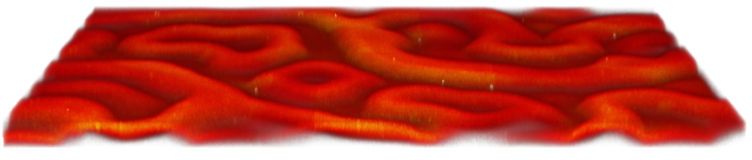
\includegraphics[width=0.4\mylength]{recol_volume_plis}};
	\end{tikzpicture}

\end{textblock}

\begin{textblock}{15}(0,8)
	\Head{Initial flat contact with a substrate: Poroelastic blistering}
	
\end{textblock}

\begin{textblock}{3}(0,8.5)
	\begin{tikzpicture}
	\matrix[matrix of nodes, matrix anchor=north east, inner sep=0, row sep=0.01\textwidth]  (m){
	
\includegraphics[width=\columnwidth, height=0.061\columnwidth]{coupe_cloque_t000.png}\\
	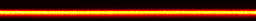
\includegraphics[width=\columnwidth, height=0.061\columnwidth]{coupe_cloque_t011.png}\\
	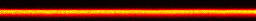
\includegraphics[width=\columnwidth, height=0.061\columnwidth]{coupe_cloque_t110.png}\\
	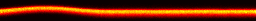
\includegraphics[width=\columnwidth, height=0.061\columnwidth]{coupe_cloque_t116.png}\\
	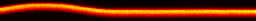
\includegraphics[width=\columnwidth, height=0.061\columnwidth]{coupe_cloque_t117.png}\\
	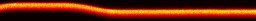
\includegraphics[width=\columnwidth, height=0.061\columnwidth]{coupe_cloque_t123.png}\\
	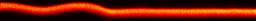
\includegraphics[width=\columnwidth, height=0.061\columnwidth]{coupe_cloque_t200.png}\\
	
\includegraphics[width=\columnwidth, height=0.061\columnwidth]{coupe_cloque_t221.png}\\
	};
	\begin{scope}[above left, white, fill=gray]
		\node at (m-1-1.south east) {\SI{15}{\minute}};
		\node at (m-2-1.south east) {\SI{22}{\minute}};
		\node at (m-3-1.south east) {\SI{1}{\hour}~26};
		\node at (m-4-1.south east) {\SI{1}{\hour}~30};
		\node at (m-5-1.south east) {\SI{1}{\hour}~31};
		\node at (m-6-1.south east) {\SI{1}{\hour}~35};
		\node at (m-7-1.south east) {\SI{2}{\hour}~25};
		\node at (m-8-1.south east) {\SI{2}{\hour}~40};
	\end{scope}
	\draw[<->, ultra thick] ($(m-8-1.south west)+(0,-0.25em)$) -- +(0.786\textwidth,0) node[midway, below] {\SI{1}{\milli\metre}};
	\end{tikzpicture}
	
	\begin{tikzpicture}
	\begin{groupplot}[%
		group style={
			group name=g, group size=1 by 2,
			xticklabels at=edge bottom,
			vertical sep=0,
			},
		xmin=0, xmax=170, xtick={0,30,...,150},
		extra tick style={grid=major},%
		extra x tick labels={},%
		scale only axis,
		width=\textwidth-4em,
		height=0.3\textwidth,
		ylabel absolute, every axis y label/.append style={anchor=base, yshift=1.25em}
		]
	
	\nextgroupplot[ylabel={Volume (\%)}, ymin=20, ymax=100, ytick={40,60,80,100}, every axis y label/.append style={xshift=0.5em}]
	\addplot+[no marks,Accent1] table[x expr={\thisrowno{0}+15}, y expr={\thisrowno{1}*100}]{relative_volume_excess_area_cloques.txt};
	%\addplot+[only marks,Accent2, mark=+] table[y expr={\thisrowno{1}*100}]{volume_rel_half_cas8_toi.txt};
	
	\nextgroupplot[ylabel={Excess area (\%)}, ymin=0, ymax=2, ytick={0,0.5,1,1.5}, xlabel={time (min)}, every axis y label/.append style={xshift=-1em}]
	\addplot+[no marks,Accent1] table[x expr={\thisrowno{0}+15}, y expr={\thisrowno{2}*100}]{relative_volume_excess_area_cloques.txt};
	%\addplot+[only marks,Accent2, mark=+] table{excess_area_pc_half_cas8_toi.txt};
	\end{groupplot}
	\end{tikzpicture}
	
\end{textblock}

\begin{textblock}{3}(4,8.5)
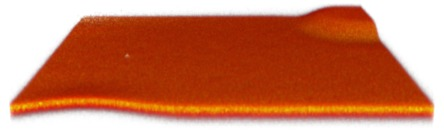
\includegraphics[width=\textwidth]{volume_cloque_t116.jpg}

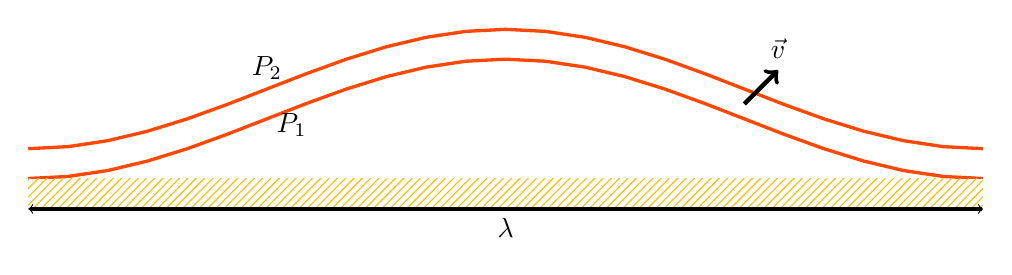
\begin{tikzpicture}[ultra thick]
\begin{axis}[
	name=a,
	width=\textwidth, height=0.25\textwidth, scale only axis,
	domain=-180:180, no markers, ymin=0, ymax=4,xmin=-180,xmax=180,
	axis lines=none, xtick=\empty,
	]
	\addplot+[Accent1]{cos(x)+1};
	\addplot+[Accent1]{cos(x)+1.5};
	\draw[->, ultra thick] (axis cs:90,1.25) -- +(45:0.05\textwidth) node[pos=1, above] {$\vec{v}$};
	\node[above] at (axis cs:-90,1.5) {$P_2$};
	\node[below right] at (axis cs:-90,1.25) {$P_1$};
\end{axis}
\fill[pattern=north east lines,pattern color=Accent2] (a.south west) rectangle (\textwidth,-1em);
\draw[<->] ($(a.south west)+(0,-1.1em)$) -- +(\textwidth,0) node[midway, below] {$\lambda$};
\end{tikzpicture}

\begin{itemize}
\item Synæresis then swelling
\item First blister after $\approx\SI{1}{\hour}$ of swelling
\item Independent blisters
\item $\lambda \ll L \Rightarrow$ not buckling
\item Once in contact with ceiling, $\lambda$ fixed
\item Cascade buckling\linebreak \hfill\textit{Roman \& Pocheau 1999}
\end{itemize}
\end{textblock}

\begin{textblock}{3}(8,8.5)
Bending energy $B$ vs vertical stress $\sigma$:
\[ \lambda^* = \left(\frac{B}{\sigma}\right)^{1/3}\text{, eg. }\sigma =\rho g h \]
\textit{Kolinski et al 2009, Vella et al 2009}

Here $\sigma$ is a Darcy pressure due to solvent flow through the gel (pore size $\ell_p$)
\[\sigma = \Delta P \sim \eta h v/\ell_p^2   \]
\end{textblock}


\begin{textblock}{15}(0,14)
	\Head{No initial contact with a substrate: Poiseuille vs Darcy on a flying carpet}
	\begin{tikzpicture}
	\matrix[matrix of nodes, inner sep=0, column sep=0.015\textwidth, row sep=0.5em] (m){
	33 min & 38 min & 43 min & 48 min & 1h & 1h15 & 2h30\\
	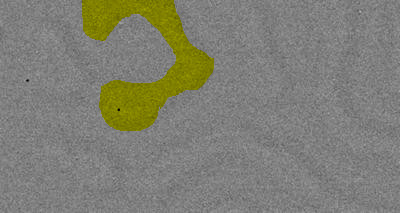
\includegraphics[width=0.13\textwidth]{prise_0100_color.jpg}&
	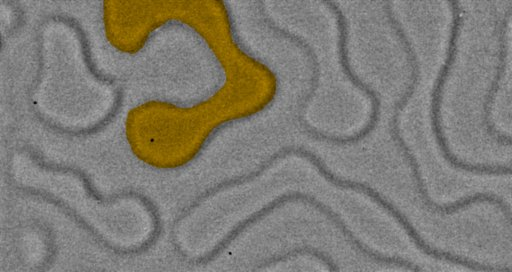
\includegraphics[width=0.13\textwidth]{prise_0130_color.jpg}&
	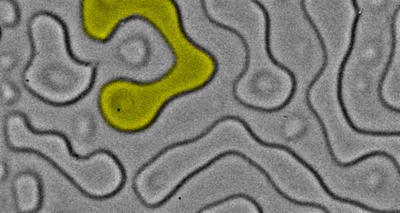
\includegraphics[width=0.13\textwidth]{prise_0160_color.jpg}&
	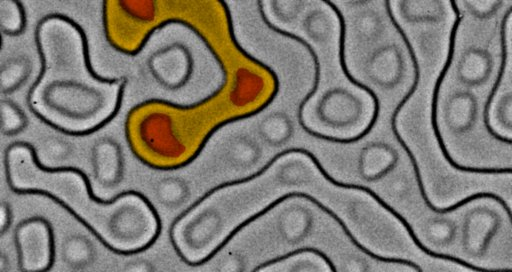
\includegraphics[width=0.13\textwidth]{prise_0190_color.jpg}&
	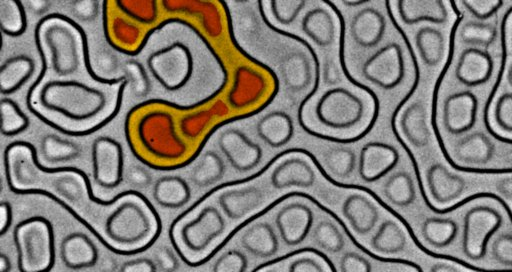
\includegraphics[width=0.13\textwidth]{prise_0250_color.jpg}&
	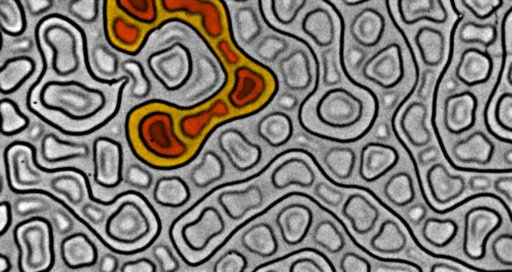
\includegraphics[width=0.13\textwidth]{prise_0360_color.jpg}&
	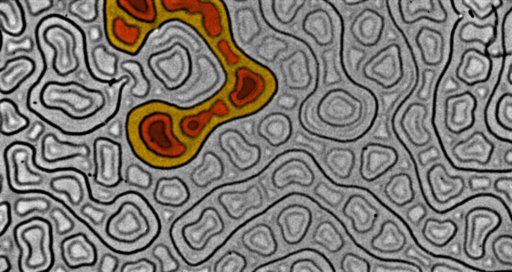
\includegraphics[width=0.13\textwidth]{prise_0799_color.jpg}\\
	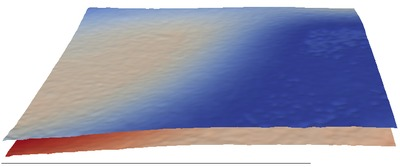
\includegraphics[width=0.13\textwidth]{cas3p2_fluo0p8_GDL4_2_t047_crop_resized.jpg}&
	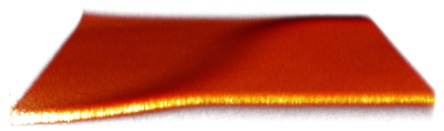
\includegraphics[width=0.13\textwidth]{cas3p2_fluo0p8_GDL4_2_t056_crop_resized.jpg}&
	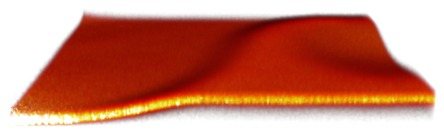
\includegraphics[width=0.13\textwidth]{cas3p2_fluo0p8_GDL4_2_t065_crop_resized.jpg}&
	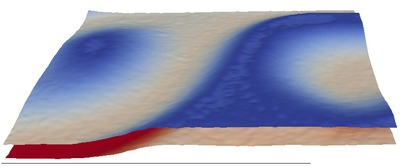
\includegraphics[width=0.13\textwidth]{cas3p2_fluo0p8_GDL4_2_t074_crop_resized.jpg}&
	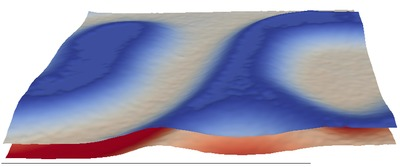
\includegraphics[width=0.13\textwidth]{cas3p2_fluo0p8_GDL4_2_t092_crop_resized.jpg}&
	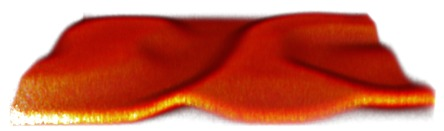
\includegraphics[width=0.13\textwidth]{cas3p2_fluo0p8_GDL4_2_t125_crop_resized.jpg}&
	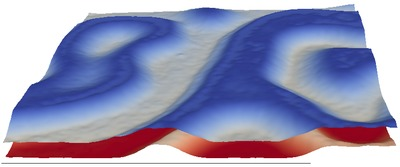
\includegraphics[width=0.13\textwidth]{cas3p2_fluo0p8_GDL4_2_t260_crop_resized.jpg}\\
	};
	\draw[ultra thick] ++(m-2-1.south west) -- ++(0.023\textwidth,0);
	\draw[ultra thick] ++(m-3-1.south west) -- ++(0.1\textwidth,0);
	\end{tikzpicture}
\end{textblock}






\begin{textblock}{15}(0,25)
\small{\texttt{The research leading to these results has received funding from the European Research Council under the European Union's Seventh Framework Programme (FP7/2007-2013) / ERC grant agreement n°~258803.}}
\end{textblock}


\textblockcolour{lightgray!50!white}
\TPMargin*{ 0.125\TPHorizModule }
\begin{textblock}{2.875}(12,2.625)%real width of 3
	\Norulehead{Take home}
	\Subhead{Poroelasticity dominates}
	\begin{itemize}
		\item gravity
		\item lubrication
	\end{itemize}
	\Subhead{Two modes}
	\begin{itemize}
		\item blistering
		\item wrinkling
	\end{itemize}
	\Subhead{Nested patterns}
	\begin{itemize}
		\item generated by swelling
		\item kinetic wavelength
	\end{itemize}

\end{textblock}%Conclusion



\end{document}